\documentclass[twoside,11pt]{article}

\usepackage{../Style/feuille-tp}

\formation{IUT - Département Informatique}
\matiere{Théorie des langages}
\titre{Devoir de rattrapage}
\sigle{Maths \\ 2013-2014}


\sloppy

\begin{document}


\maketitle

\textbf{Sans documents, durée 1h}

%\begin{multicols*}{2}


\section{Automates}

\Q Donnez un automate qui reconnait les mots sur $A  = \{ a, b \}$ qui ont \emph{au moins} un $a$.

\Q Même question pour les mots qui ont \emph{au plus} un $b$.

\Q En utilisant comme exemples les automates ci-dessus, montrez 
comment construire un automate qui reconnait l'intersection de deux
langages rationnels, à partir de leurs automates respectifs.



\section{Expressions régulières}

Donnez une expression régulière pour le langage reconnu par l'automate 
ci-dessous \begin{center}
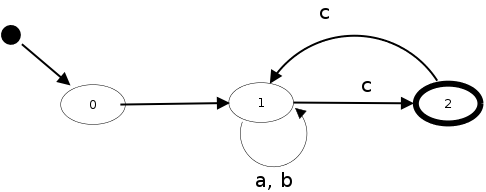
\includegraphics[width=0.5\linewidth]{../dia/auto-ds-rattrapage}
\end{center}

\section{Grammaire et dérivation}

Soit la grammaire $\mathcal{G}$ ci-dessous, d'axiome $S$ 
$$\begin{array}{rcl}
S & \rightarrow &a S b \\
S & \rightarrow & b S a  \\
S & \rightarrow & \epsilon 
\end{array}
$$

\Q Donnez l'arbre de dérivation du mot $ababab$

\Q Montrez que le mot $aababbababbabb$ n'appartient pas au langage
reconnu par   $\mathcal{G}$.

\section{Un langage algébrique}

\Q Donnez une grammaire pour le langage
$ L = \{ a^n b^p, 0 \leq n \leq p \}$
% \end{multicols*}
\end{document}
